\documentclass[11pt,a4paper]{book}
\textwidth 170 mm
\textheight 250 mm
\topmargin -15 mm
\oddsidemargin -5 mm
\evensidemargin -5 mm

\newcounter{ProblemNo}
\setcounter{ProblemNo}{0}
\def\tempID{0}
%\def\UndAns{} %% <-------------- Uncomment in final version!!
\def\UndAns{\underline}
\def\UndAns{\underline}
\newcommand{\ZOdg}[1]{}
\def\text{}
%\def\dfrac{\displaystyle\frac}

\usepackage{amsfonts,amssymb,amsmath}
\usepackage{graphicx}
\DeclareGraphicsExtensions{.pdf,.PDF,.png,.PNG} % prefer pdf to png
\usepackage{etoolbox}
\usepackage{sidepicture}
\newcommand{\problemID}[3]{\def\tempID{#1 (#3)}\ignorespacesafterend}
%\newcommand{\problemID}[3]{\def\tempID{#1}\noindent{\bf #1, #2}\par}
%\newcommand{\problemID}[3]{\def\tempID{#3: \##1}\par}
%\newcommand{\problemRating}[3]{{\bf #1, #2, #3}\par}
%\newcommand{\problemID}[3]{\def\tempID{\# #1}\par}
%\newcommand{\problemRating}[3]{}
%\newcommand{\xProblem}[8]{#1\par (A) #2\quad (B) #3\quad  (C) #4\quad  (D) #5\quad (E) #6\par Correct: #7\bigskip\bigskip\par }

%\usepackage{xcolor}
%\usepackage{everypage}
%\usepackage[absolute]{textpos}
%\usepackage{rotating}
%\AddEverypageHook{\begin{textblock*}{2.5cm}(0.7cm,5cm)\begin{turn}{90}{\color{red}\Huge\sc Solutions included - do not use for contest}\end{turn}\end{textblock*}}

\newcommand{\Problem}[9]
{%\newpage
%\noindent\addtocounter{ProblemNo}{1}{\bf\arabic{ProblemNo}.\hspace{3pt}~}%
\noindent\addtocounter{ProblemNo}{1}{\bf\tempID.\hspace{3pt}~}%
\edef\answer{{#7}}\def\SettingMode{#8}%
\def\VLine{\vrule height14pt width0pt\quad}#1\nopagebreak\vspace{1ex}\newline%
\VLine\expandafter\ifstrequal\answer{A}{\UndAns{(\rlap{\bf A}\phantom{\bf C})}\ZOdg{A}}{(\rlap{\bf A}\phantom{\bf C})}\nolinebreak\hspace{3pt}%
\ifnum\SettingMode=3{#2}\else\rlap{#2}\fi\quad\ifnum\SettingMode=3\newline\VLine\else\hfil\fi%
\expandafter\ifstrequal\answer{B}{\UndAns{(\rlap{\bf B}\phantom{\bf C})}\ZOdg{B}}{(\rlap{\bf B}\phantom{\bf C})}\nolinebreak\hspace{3pt}%
\ifnum\SettingMode=3{#3}\else\rlap{#3}\fi\quad\ifnum\SettingMode=2\newline\VLine\else\ifnum\SettingMode=3\newline\VLine\else\ifnum\SettingMode=6{\phantom{({\bf C})}\quad\hspace{6pt}\hfil\hfil\newline\VLine}\else\hfil\fi\fi\fi%
\expandafter\ifstrequal\answer{C}{\UndAns{(\rlap{\bf C}\phantom{\bf C})}\ZOdg{C}}{({\bf C})}\nolinebreak\hspace{3pt}%
\ifnum\SettingMode=3{#4}\else\rlap{#4}\fi\quad\ifodd\SettingMode\newline\VLine\else\hfil\fi%
\expandafter\ifstrequal\answer{D}{\UndAns{(\rlap{\bf D}\phantom{\bf C})}\ZOdg{D}}{(\rlap{\bf D}\phantom{\bf C})}\nolinebreak\hspace{3pt}%
\ifnum\SettingMode=3{#5}\else\rlap{#5}\fi\quad\ifnum\SettingMode>1\ifnum\SettingMode<6\newline\VLine\else\hfil\fi\else\hfil\fi%
\expandafter\ifstrequal\answer{E}{\UndAns{(\rlap{\bf E}\phantom{\bf C})}\ZOdg{E}}{(\rlap{\bf E}\phantom{\bf C})}\nolinebreak\hspace{3pt}%
\ifnum\SettingMode=3{#6}\else\rlap{#6}\fi\quad\ifnum\SettingMode=1\hfil\phantom{({\bf C})}\fi\hspace{3pt}\hfil\par\vspace{2ex}\par\noindent{\sc Solution: }#9\bigskip}


\def\TheHead{Benjamin Finalized}
\makeatletter
\def\ps@pKSF{
\def\@oddfoot{\hfill{\rm \thepage}\hfill}\def\@evenfoot{\hfill{\rm \thepage}\hfill}
\def\@oddhead{\hfill{\em \TheHead}\hfill}\def\@evenhead{\hfill{\em \TheHead}\hfill}
}
\makeatother 
\pagestyle{pKSF}

\begin{document}

\noindent{\large\bf Benjamin}\bigskip

\noindent\fbox{3 points}\bigskip

\problemID{1}{20197}{Iran}%
\problemRating{B}{3}{G}%
\Problem{Alina folds the image below along the dashed line.\newline
\centerline{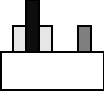
\includegraphics{B01-1}}\newline
Which of the following squares folds onto an identical one?}
{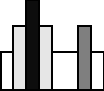
\includegraphics{B01-2}}{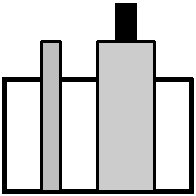
\includegraphics{B01-3}}{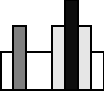
\includegraphics{B01-4}}{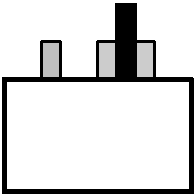
\includegraphics{B01-5}}{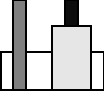
\includegraphics{B01-6}}
{B}{0}
{coloured version: \includegraphics{B01-7}
\newline
\includegraphics{B01-8}}

\NSidePictureEPS[yoffset=-17.5ex]{B02-1}{\problemID{2}{20198}{Austria}%
\problemRating{B}{3}{N}%
\Problem{The picture shows the first few squares of a hopping game. Every fourth square in the game has the same image in it. Mia is playing the game. In which of the following squares will Mia land only on her right foot?}
{the 10th}{the 15th}{the 20th}{the 22nd}{the 23rd}
{C}{0}
{Mia lands on the fourth field with only the left foot, the pattern repeats after these four jumps. So, she hops in all fields which are a multiple of 4 with only the left foot. As $20$ Is the multiple of four among the options, it must be the solution.}}

\problemID{3}{20199}{Uzbekistan}%
\problemRating{B}{3}{L}%
\Problem{Sasha created a secret alphabet. He writes ``basil'' as  \includegraphics[scale=0.6]{B03-3}  and ``red'' as \includegraphics[scale=0.6]{B03-4} . How does he write ``bread''?}
{\includegraphics[scale=0.6]{B03-5}}{\includegraphics[scale=0.6]{B03-6}}{\includegraphics[scale=0.6]{B03-7}}{\includegraphics[scale=0.6]{B03-8}}{\includegraphics[scale=0.6]{B03-9}}
{C}{0}
{The word  ``basil'' starts with a 
\includegraphics[scale=0.6]{B03-10}. The word ``bread'' starts as well with a 
\includegraphics[scale=0.6]{B03-10}. Answer C is the only one starting with 
\includegraphics[scale=0.6]{B03-10}, so it must be the correct answer.}

\NSidePictureEPS[scale=1.1]{B04-6}{\problemID{4}{20200}{Catalonia}%
\problemRating{B}{3}{L}%
\Problem{Which of the strips should be placed in the space in the picture so that each child is connected to a different kite?}
{\includegraphics{B04-1}}{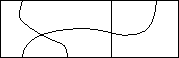
\includegraphics{B04-2}}{\includegraphics{B04-3}}{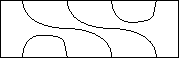
\includegraphics{B04-4}}{\includegraphics{B04-5}}
{D}{2}
{\includegraphics{B04-7}}}

\problemID{5}{20201}{Switzerland}%
\problemRating{B}{3}{G}%
\Problem{Dina has set up her three bricks on the floor behind a wall. 
When seen from the front, the bricks look like this
\includegraphics{B05-1}.

How do the bricks look from the back ?}
{\includegraphics{B05-2}}{\includegraphics{B05-3}}{\includegraphics{B05-4}}{\includegraphics{B05-5}}{
\includegraphics{B05-6}}
{B}{0}
{If you look from the back:
- the three bricks stand before the wall, so it can't be answer D.
- the two bricks are now on the right-hand side, so in can't be answer A.
- the light grey block stands in front of the dark grey block, so it can't be answer C.
Of the two thin bricks, the dark grey stick is longer than the light grey stick, so the correct answer is B.}

\NSidePictureEPS{B06-1}{\problemID{6}{20202}{Germany}%
\problemRating{B}{3}{L}%
\Problem{Mona wants to draw the figure shown without lifting up her pencil from the paper.
The lengths of the three segments are given.
What is the shortest total length she could draw?}
{$6 \textup{cm}$}{$7 \textup{cm}$}{$8 \textup{cm}$}{$9 \textup{cm}$}{$10 \textup{cm}$}
{B}{0}
{The shortest total distance is $3 \textup{ cm} + 2 \cdot 1 \textup{ cm} + 2 \textup{ cm} = 7 \textup{ cm}$.
\newline
\includegraphics{B06-2}}}

\problemID{7}{20203}{Mexico}%
\problemRating{B}{3}{N}%
\Problem{There are 2 wheels each marked with 7 positions. The wheels spin in opposite directions and each makes a complete turn in seven minutes. At the end of each minute, each letter lies exactly in front of a number. The picture shows the first two positions of the wheels and we can see that initially letter $A$ is in front of number 1,  letter $B$ is in front of number 2, and so on. The wheels turn until letter  $C$ is in front of number 2. Which number is letter $F$ in front of that point?\newline
\centerline{\includegraphics[scale=1]{B07-1}}}
{1}{4}{5}{6}{7}
{C}{0}
{Instead of both wheels moving, we can imagine that the outer wheel is fixed and only the inner wheel turns, but not one, but two positions in anti-clockwise direction.
We can observe what happens with the letter $C$. It starts in front of number 3, after one minute it is in front of number 1 (as seen in the problem), after two minutes it is in front of number 6, after three minutes in front of number 4 and after four minutes in front of number 2!  
What happens with the letter $F$? Letter $F$ also moves two position anti-clockwise every minute. It starts in front of number 6, after 1 minute it is in front of number 4, after 2 minutes it is in front of number 2, after 3 minutes in front of number 7 and if 4 minutes in front of number 5. So, the correct answer is C.}

\problemID{8}{20204}{Greece}%
\problemRating{B}{3}{L}%
\Problem{There are six boxes on a truck as shown.\newline
\centerline{\includegraphics[scale=0.8]{B08-1}}\newline
A worker puts them on the floor. He takes one box at a time, provided that  box does not have another box on top of it. He places his box on the ground or on top of another box. Which of the following stacks could he not build?}
{\includegraphics[scale=0.8]{B08-2}}{\includegraphics[scale=0.8]{B08-3}}{\includegraphics[scale=0.8]{B08-4}}{\includegraphics[scale=0.8]{B08-5}}{\includegraphics[scale=0.8]{B08-6}}
{C}{0}
{Box  D cannot be above B so the third picture is impossible.  It is easy to see that all other cases are possible.}

\problemID{9}{20205}{Poland}%
\problemRating{B}{3}{N}%
\Problem{Pieter has a package of $445\ \textup{g}$ and the following eight weights:
\newline
\centerline{\includegraphics{B09-1}}
\newline
He put the package on the scale, as shown.
What is the minimum number of weights he needs to balance the scale?
\newline
\centerline{\includegraphics{B09-2}}
\newline
\newline}
{\(2\)}{\(3\)}{\(4\)}{\(5\)}{\(6\)}
{B}{0}
{All you need is three: put one weight of 500 g on one pan, and the package and one weight of 50 g and 5 g each on the other pan.}

\problemID{10}{20206}{Slovakia}%
\problemRating{B}{3}{N}%
\Problem{The rooms in the hotel are numbered in ascending order, starting from 1. No number is omitted. Kangaroo counted the digits in the rooms and found digit 2 14 times and digit 5 3 times. What is the largest number of rooms there can be in the hotel?}
{25}{26}{34}{35}{41}
{C}{0}
{With the 14 digits 2 the rooms 2, 12, 20, 21, 22, 23, 24, 25, 26, 27, 28, 29 and 32 can be numbered. The first room that can't be numbered is in this case room 42.
With the 3 digits 5 the rooms 5, 15 and 25 can be numbered. The first room that can't be numbered is in this case room 35.
So, answer C is correct, at most 34 room can be numbered with the digits given.}

\noindent\fbox{4 points}\bigskip

\problemID{11}{20207}{Norway}%
\problemRating{B}{4}{N}%
\Problem{Two identical rectangles, each with an area of 18, overlap to form a new rectangle, as shown. The new rectangle can be divided into three identical squares.
\newline
\centerline{\includegraphics{B11-1}}\newline
What is the area of the new rectangle?\newline
\newline}
{24}{27}{30}{32}{36}
{B}{0}
{The two rectangles have a total area of $36$. When they overlap to form the three identical squares, the overlap is the half of one rectangle. So, the total area is reduced by $9$, it is $36 - 9 = 27$, the correct answer is B.}

\problemID{12}{20208}{Greece}%
\problemRating{B}{4}{L}%
\Problem{A student had five boxes of chocolates labelled $A$, $B$, $C$, $D$ and $E$. The chocolates in the boxes have been given numbers according to their flavour, as shown.\newline
\centerline{\includegraphics{B12-1}}\newline
He ate most of the chocolates. The picture below shows what was left. What was the label of the box marked $X$?\newline
\centerline{\includegraphics{B12-2}}}
{A}{B}{C}{D}{E}
{E}{0}
{Box $U$ has a $1$, and there is only one box with a $1$, namely $A$. So $U=A$. Now look at $W$ which has a $2$. There are two boxes with a $2$, namely $A$ and $B$, and $A$ is already used. So $W=B$. Similarly, there are three boxes with a $3$, namely $A$, $B$, $C$, but $A$ and $B$ are already used. So $Z=C$. Similarly, $Y=D$ and finally $X=E$.\newline
\includegraphics{B12-3}}

\problemID{13}{20209}{Malaysia}%
\problemRating{B}{4}{G}%
\Problem{Rosa draws several identical rectangles to make the following picture. The width and the height of the picture are $45\ \text{cm}$ and $30\ \text{cm}$ respectively. What is the area of one rectangle?
\newline
\centerline{\includegraphics{B13-1}}}
{$24\ \text{cm}^2$}{$27\ \text{cm}^2$}{$30\ \text{cm}^2$}{$33\ \text{cm}^2$}{$36\ \text{cm}^2$}
{E}{0}
{The structure is $45\ \text{cm}$ wide, this corresponds to the length of five bricks. So, one brick is $9\ \text{cm}$ long. The height of the structure is $30\ \text{cm}$. It consists of the the length of two bricks, this is in total  $18\ \text{cm}$ and the width of three rectancles. So, the three widhts add up to the missing $12\ \text{cm}$ of the height. This means that each brick is $4\ \text{ cm}$ wide. So, the area of a brick is $9\ \text{cm} \cdot 4\ \text{cm} = 36\ \textup{cm}^2$. So, the correct answer is E.}

\problemID{14}{20210}{Greece}%
\problemRating{B}{4}{N}%
\Problem{Each of the 16 circles shown contains a number. Numbers in neighbouring circles differ by 1. One of the circles contains the number 5 and another one contains 13. How many different numbers are written in the 16 circles?\newline
\centerline{\includegraphics{B14-1}}}
{9}{10}{13}{14}{16}
{A}{0}
{From 5 to 13 there are 7 integers in between, which is exactly the same number as the number of circles between a given circle and the one diametrically opposite. So these in between circles MUST contain the seven numbers 6, 7, 8, 9, 10, 11, 12. This is true for either side between the circle with the 5 and the diametrically opposite with the 13. In other words the numbers in the circles between 5 and 13 are uniquely determined. The figure shows the completed figure, The numbers that appear are 5 to 13. Nine of them.\newline
\includegraphics{B14-2}}

\problemID{15}{20211}{China}%
\problemRating{B}{4}{G}%
\Problem{The diagram shows two large squares with the same area. Part of each square is shaded, as shown. In the first square, the midpoints of adjacent sides are joined. In the second square, four smaller squares all with side-lengths equal to a third of the side-lenght of the large squrare are shaded. The area shaded in the first square is $9$. What is the area shaded in the second square?
\newline
\centerline{\includegraphics{B15-1}}}
{4}{8}{9}{10}{12}
{B}{0}
{The square on the left can be divided into four smaller identical squares as shown in the figure above. In each of these small squares, the half of the square is shaded. So, the area of the big square is $18$.
The square at the right hand side can be divided up in $9$ identical squares. Four of them are shaded, so the total shaded area in the square on the right is $18 : 9 \cdot 4 = 8$. The correct answer is B.
\newline
\includegraphics{B15-2}}

\problemID{16}{20212}{Russia}%
\problemRating{B}{4}{A}%
\Problem{The Braille system for blind people, when written down, has the digits 0 to 9 represented by a set of black or white dots, as shown. \newline
\centerline{
\includegraphics[scale=0.7]{B16-1}} \newline
How many different two-digit numbers contain exactly five black dots?}
{16}{18}{30}{32}{34}
{C}{0}
{Numbers are two-digit. So 2 black points could be on the first place and 3 points could be on the second place. It is $4 \cdot 4 = 16$ options. Also it could be 3 points (exception of 0) on the first place and 2 points on the second place. It is $3 \cdot 4 = 12$ options. Also it could be combination of 1 and 4 points. It is number 17 and 71. There are $16 + 12 + 2 = 30$ numbers in total.}

\problemID{17}{20213}{Turkey}%
\problemRating{B}{4}{L}%
\Problem{The figure below shows a beehive with 16 cells. Some of the cells contain honey. The number in each cell indicates how many of its neighbouring cells contain honey. Two cells are neighbours if they share a common edge. How many cells in the beehive contain honey? \newline
\centerline{\includegraphics{B17-1}}}
{7}{8}{9}{10}{11}
{C}{0}
{\includegraphics{B17-2}}

\problemID{18}{20214}{Greece}%
\problemRating{B}{4}{N}%
\Problem{Annie wants to place the numbers 1 to 10 in the circles in the diagram with one number in each circle. She wants the sum of the numbers in any four circles that are in a straight line, for example the four grey ones, to be 23. What number must she place in the circle containing the question mark?\newline
\centerline{\includegraphics{B18-1}}}
{4}{5}{6}{7}{8}
{D}{0}
{The sum of all numbers in the circles is $1+2+...+10=55$. If we add the numbers in the three straight lines we get $3\times 23=69$. But this is because the number at the upper circle counted three times. The extra two account for the excess $69-55=14$. So in this circle the number $14\div 2=7$ is placed.
If we want an example to show that the situation is not fictitious, the following would do: $7+1+6+9=7+3+5+8=7+2+4+10$.}

\problemID{19}{20215}{Iran}%
\problemRating{B}{4}{G}%
\Problem{Christian has cut four small squares from the corners of the larger square, so that the remaining area is half of the area of the original square. The side-lenghts of the small squares are shown in the diagram. \newline
What is the perimeter of the remaining shape? \newline
\centerline{\includegraphics{B19-1}}}
{36}{40}{44}{48}{52}
{B}{0}
{The total cut area is $50 = 36 + 9 + 4 + 1$. So, the original square's area was 100, and its perimeter, which is the same as the remaining shape's perimeter, is 40.}

\problemID{20}{20216}{Norway}%
\problemRating{B}{4}{L}%
\Problem{Ria wants to complete the puzzle shown so that each row and each column contain the numbers 1, 2, 3 and 4 exactly once. She wants to place the numbers so that the greater than and less symbols ($>$ and $<$) give a correct relationship between the two values either side of them. The symbols work in all directions, as shown in the example: \newline
\centerline{\includegraphics{B20-1}}\newline
What number should she place in the gray circle?\newline
\centerline{\includegraphics{B20-2}}}
{1}{2}{3}{4}{2 or 3}
{A}{0}
{\includegraphics{B20-3}}

\noindent\fbox{5 points}\bigskip

\NSidePictureEPS{B21-1}{\problemID{21}{20217}{Slovakia}%
\problemRating{B}{5}{L}%
\Problem{There are three identical special dice on the table. What is the sum of the numbers on the faces that touch the table?}
{26}{40}{43}{47}{56}
{C}{0}
{At the first die, if you look at the number 22, so that it is in a "normal" position, at the right of 22 is the number 34. The number we are trying to find is on the left of 22. At  the last die we can see, that the number 13 is on the left of 22.
At the second die, the number 5 is positioned "above" the number 13. We are trying to find the number that is "below" 13. At the third die we can see, that the number 22 is below 13.
At the third die, the number 17 is positioned "above" the number 22. We are trying to find the number that is "below" 22. At the first die we can see, that the number 8 is below 22.
So, the correct solution is $13 + 8 + 22 = 43$, this is answer C.}}

\problemID{22}{20218}{Myanmar}%
\problemRating{B}{5}{G}%
\Problem{The diagram shows four touching rectangles. What is the area of the shaded rectangle? \newline
\centerline{\includegraphics{B22-1}}}
{$12\ \textup{cm}^2$}{$14\ \textup{cm}^2$}{$16\ \textup{cm}^2$}{$18\ \textup{cm}^2$}{$20\ \textup{cm}^2$}
{E}{0}
{\includegraphics{B22-2}\newline
Length of $a = 45 \div 5 = 9$, Length of $b = 13 - 9 = 4$, Length of $c = 40 \div 4 = 10$, Length of $d = 16 - 10 = 6$, Length of $e = 48 \div 6 = 8$, Length of $f = 8 - 4 = 4$, Length of $g = 10 - 5 = 5$. Therefore, the area of the shaded region is $4 \times 5 = 20\ \textup{cm}^2$.}

\problemID{23}{20219}{Greece}%
\problemRating{B}{5}{L}%
\Problem{The figure shows the plan of the seven train routes of a small town. The circles indicate the stations. Martin wants to paint the lines in such a way that if two lines share a common station, then they are painted with different colours. What is the smallest number of colours that he can use? \newline
\centerline{\includegraphics{B23-1}}}
{3}{4}{5}{6}{7}
{A}{0}
{There are places like the one marked as A (also B or C) that each of three lines meets the other two. Here it is lines 1, 2 and 4. For these we need 3 colours, so for the whole map we need 3 or more colours. We show that 3 are actually enough. All we have to do is to paint the lines with these colours. For example, line 6 meets both 1 and 2, so it must be the third colour. The same goes for line 5. Then we can decide the colour of 7 as it meets 1 and 5. And finally it is easy to determine the colour of line 3 as it meets lines 5 and 6.\includegraphics{B23-2}}

\problemID{24}{20220}{Germany}%
\problemRating{B}{5}{G}%
\Problem{Dimitri wants to fold the net shown to make a cube.\newline
He wants the triangles that touch the edges of neighbouring faces of the cube to be shaded the same. How should he shade the triangles of the unshaded square in the net?\newline
\centerline{\includegraphics{B24-7}}}
{\includegraphics{B24-8}}{\includegraphics{B24-9}}{\includegraphics{B24-10}}{\includegraphics{B24-11}}{\includegraphics{B24-12}}
{B}{0}
{coloured version: \includegraphics{B24-1}
\includegraphics{B24-2} \includegraphics{B24-3} \includegraphics{B24-4} \includegraphics{B24-5} \includegraphics{B24-6}
\newline
\includegraphics{B24-13}\includegraphics{B24-14}}

\problemID{25}{20221}{Germany}%
\problemRating{B}{5}{L}%
\Problem{Simon takes four cups out of the cupboard and puts them randomly on the four saucers. Which statement is correct?\newline
\centerline{\includegraphics{B25-1}}}
{It is certain that none of the 4 cups stands on its matching saucer.}{It is certain that exactly 1 cup stands on its matching saucer.}{It is impossible for exactly 2 cups to stand on its matching saucer.}{It is impossible for exactly 3 cups to stand on its matching saucer.}{It is impossible for all 4 cups to stand on its matching saucer.}
{D}{3}
{If 3 cups stand on its matching saucer then the 4th one has to stand on its matching saucer as well. Hence, it is impossible for exactly 3 cups to stand on its matching saucer.}

\NSidePictureEPS[yoffset=-7.5ex]{B26-1}{\problemID{26}{20222}{Catalonia}%
\problemRating{B}{5}{N}%
\Problem{A cube with the filled in numbers is given. Mary wants to write the numbers 1 to 8 on the vertices of the cube. She wants  the sum of the numbers of the vertices around each face to be the same. She has already written the numbers  6, 7 and 8, as shown. What number should she write on the vertex marked with the questionmark?}
{1}{2}{3}{4}{5}
{C}{0}
{The sum of all numbers is $1+2+3+4+5+6+7+8=36$. If you consider the four numbers on any face, there are four numbers on the other face left. So, the sum of the numbers on one face has to be $36:2=18$.
First, we consider the face at the right-hand side: $8+7=15$, the two remaining numbers have to be 1 and 2.
First, we consider the face at the bottom: $8+6=14$, the two remaining numbers have to be 1 and 3. So, the number in the lower right corner must be 1, consequently the number 3 is at the question mark. The correct answer is C.
\newline
\includegraphics{B26-2}}}

\problemID{27}{20223}{Catalonia}%
\problemRating{B}{5}{N}%
\Problem{A grandmother has some candies. She decides to divide them up amongst her grandchildren so that each has  a bag containing same number of candies. She puts the largest possible number of candies in each bag and, when she is done, she sees that there are 20 candies in each bag and 12 candies are left over. What is the smallest possible number of candies she could have?}
{52}{232}{272}{411}{432}
{C}{0}
{There are 12 piece of candy left over, so the number of grandchildren must be bigger than 12.  To get the smallest number of candies, the number of grandchildren should be as small as possible, so there are 13 grandchildren. In each bag for these 13 grandchildren there are 20 candies, plus the 12 left over, so the total number of candies is: $13 \cdot 20 + 12 = 272$. The correct answer is C.}

\problemID{28}{20224}{Israel}%
\problemRating{B}{5}{N}%
\Problem{Dan plans to cut a rope into 12 equal pieces and marks points where he needs to cut. Muhammad plans to cut the same rope into 16 equal pieces and marks points where he needs to cut. Then Maya cuts the rope at all the marked points.
How many pieces does Maya get?}
{24}{25}{27}{28}{29}
{A}{0}
{Dan marked every $1/12$ piece of paper (used 11 points). 
Muhammad marked every $1/16$ piece of paper (used 15 points). 
They have 3 common points: $3/12=4/16$, $6/12=8/16$, $9/12=12/16$.
Then in total, Maya had $11+15-3=23$ points to cut and hence 24 pieces of paper.}

\problemID{29}{20225}{Germany}%
\problemRating{B}{5}{N}%
\Problem{Emma is playing with the seven caterpillar puzzle pieces shown.\newline
\centerline{\includegraphics{B29-1}}\newline
She wants to build a caterpillar that has one head, one tail and either one, two or three puzzle pieces in between.
How many different caterpillars could Emma build?}
{10}{14}{16}{18}{20}
{E}{0}
{There are 4 possibilities to choose the head and the tail, and then there are always the same 5 possibilities for the inner puzzle pieces.
Altogether there are $4 \cdot 5 = 20$ possibilities.\newline
\includegraphics[scale=0.9]{B29-2}}

\problemID{30}{20226}{Catalonia}%
\problemRating{B}{5}{A}%
\Problem{Ava writes a three-digit number on the whiteboard. Then Brandon writes a fourth digit to the right of the previous ones. He says ``Look! The number increased by 2024''. What digit did Brandon write?}
{2}{3}{4}{8}{9}
{D}{0}
{Ava writes the number abc. Brandon writes the number abcd. Number abcd increased number abc by 2024, that means, that $abcd - abc = 2024$. The digit a therefore has to have the value 2. This leads to digit b, which also has the value 2. To get 2024 the digit d has to be 8 and the digit c has to have the value 4. Brandon therefore writes the digit 8 as fourth digit on the right of the previous one. $2248 - 224 = 2024$.}


\end{document}